\subsection{Experimental Setup}
All experiments were performed on the ETH Leonhard cluster\footnote{\url{https://scicomp.ethz.ch/wiki/Leonhard}} using 1 GPU with 64 GB of RAM and 1 CPU. The simple baselines (SVD, SVD++, NMF, SlopeOne) were developed using Surprise \citep{Hug2020} and the neural network models (NCF, GNN, GNN + NCF, RGNN) were implemented in the PyTorch Lightning framework \citep{falcon2019pytorch} for PyTorch \citep{NEURIPS2019_9015}. The models were trained for a maximum of 60 epochs using the Adam optimizer \citep{kingma2014adam}. We assume model convergence when no improvement in validation loss was observed for 3 consecutive epochs. The model with the lowest validation loss is used as the final model.

As recommended by \citet{rendle2019difficulty}, all baselines are extensively tuned to accurately reflect true model performance. Hyperparameter tuning was done using the Optuna framework \citep{akiba2019optuna} with a sampler using a Tree-Structured Parzen Estimator \citep{bergstra2011algorithms} to suggest parameters for each trial. No pruning was used to stop unpromising trials early; all trials were completed in their entirety. The optimal hyperparameters can be found in the source code. Similarly, extensive neural architecture searches were performed for the NCF and GNN models.

For the RGNN ensemble we further optimize over the random seeds used for each model by choosing the 12 best scoring seeds. We emphasize that this is only done due to the competitive part of the model scoring and the results do not accurately reflect model performance in different environments.

\subsection{Results}
We compare the proposed RGNN model to the various baselines outlined in \autoref{baselines} as well as the GNN + NCF model. We measure model performance with the root mean square error (RMSE) on the public Kaggle dataset. Results from our experiments are summarized in \autoref{tab:results}. We observe that combining the GNN and NCF model into the GNN + NCF model yields a significant performance boost compared to the NCF and GNN baselines. Further improvements can be observed when adding reinforcements to the GNN + NCF model leading to our proposed RGNN model. The training time of the RGNN remains similar to the time of the GNN + NCF model. Employing ensemble learning to the RGNN boosts performance from an RMSE of $0.985$ to $0.982$.

\autoref{tab:results_rgnn} shows model performance by reinforcement used in our RGNN model. Adding reinforcements from the SlopeOne baseline yields the lowest RMSE of $0.9854$. In \autoref{fig:learning_curve_comparison} we further show a comparison of learning curves between our proposed RGNN model and the GNN + NCF baseline. Here we observe that the loss on the held-out validation set fluctuates less through training when reinforcements are used. Since fluctuations in the validation loss are tied to unstable predictions, we conclude that the RGNN makes more stable predictions than the GNN + NCF.

\begin{table}[]
\centering
\begin{tabular}{llr}
\hline
Method & \multicolumn{1}{l}{RMSE} & \multicolumn{1}{l}{Training time (m)} \\ \hline
NCF & $	1.024$ & $65$ \\
SVD & $1.003$ & \boldmath$2$ \\
NMF & $1.000$ & $3$ \\
GNN & $1.000$ & $9$ \\
SVD++ & $0.999$ & $185$ \\
SlopeOne & $0.998$ & $4$ \\
GNN + NCF & $0.988$ & $29$ \\
RGNN & $0.985$ & $26$ \\ 
RGNN ensemble & \boldmath$0.982$ & $437$ \\ \hline
\end{tabular}
\caption{Comparison between various baselines and our proposed RGNN method evaluated on the public Kaggle dataset.}
\label{tab:results}
\end{table}

\begin{table}[]
\centering
\begin{tabular}{ll}
\hline
Reinforcements & RMSE \\ \hline
SVD, NMF & $0.9880$ \\
SVD & $0.9875$ \\
SVD, SVD++ & $0.9875$ \\
SVD, NMF, SlopeOne & \multicolumn{1}{r}{$0.9870$} \\
SVD, SlopeOne & $0.9870$ \\
NMF, SlopeOne & \multicolumn{1}{r}{$0.9870$} \\
SlopeOne, SVD++ & \multicolumn{1}{r}{$0.9869$} \\
SVD, NMF, SVD++ & $0.9868$ \\
NMF & \multicolumn{1}{r}{$0.9868$} \\
NMF, SlopeOne, SVD++ & \multicolumn{1}{r}{$0.9864$} \\
SVD, SlopeOne, SVD++ & $0.9864$ \\
SVD++ & $0.9862$ \\
NMF, SVD++ & \multicolumn{1}{r}{$0.9861$} \\
SVD, NMF, SlopeOne, SVD++ & \multicolumn{1}{r}{$0.9859$} \\
SlopeOne & \multicolumn{1}{r}{\boldmath$0.9854$} \\  \hline
\end{tabular}
\caption{Comparison between reinforcements used in our RGNN model evaluated on the public Kaggle dataset.}
\label{tab:results_rgnn}
\end{table}

\begin{figure}
    \centering
    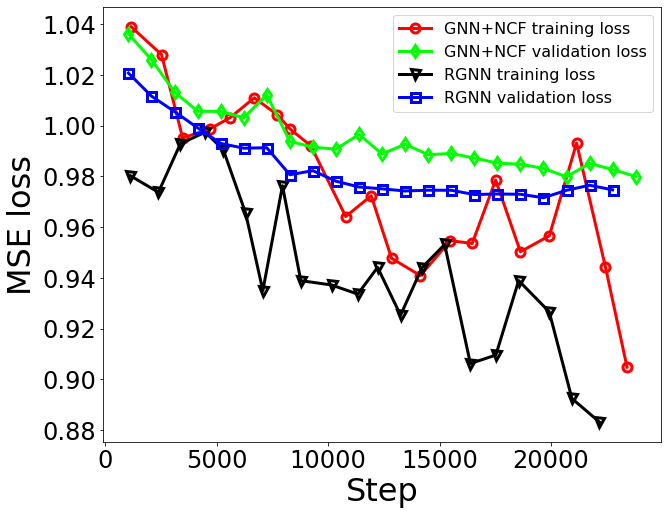
\includegraphics[width=0.45\textwidth]{figures/learning_curve.png}
    \caption{Comparison of learning curves between our RGNN model and the GNN + NCF baseline.}
    \label{fig:learning_curve_comparison}
\end{figure}